\documentclass[ignorenonframetext,]{beamer}
\setbeamertemplate{caption}[numbered]
\setbeamertemplate{caption label separator}{: }
\setbeamercolor{caption name}{fg=normal text.fg}
\beamertemplatenavigationsymbolsempty
\usepackage{lmodern}
\usepackage{amssymb,amsmath}
\usepackage{ifxetex,ifluatex}
\usepackage{fixltx2e} % provides \textsubscript
\ifnum 0\ifxetex 1\fi\ifluatex 1\fi=0 % if pdftex
  \usepackage[T1]{fontenc}
  \usepackage[utf8]{inputenc}
\else % if luatex or xelatex
  \ifxetex
    \usepackage{mathspec}
  \else
    \usepackage{fontspec}
  \fi
  \defaultfontfeatures{Ligatures=TeX,Scale=MatchLowercase}
\fi
\usetheme[]{Warsaw}
\usefonttheme{structurebold}
% use upquote if available, for straight quotes in verbatim environments
\IfFileExists{upquote.sty}{\usepackage{upquote}}{}
% use microtype if available
\IfFileExists{microtype.sty}{%
\usepackage{microtype}
\UseMicrotypeSet[protrusion]{basicmath} % disable protrusion for tt fonts
}{}
\newif\ifbibliography
\hypersetup{
            pdftitle={Progrmación en R-Introducción},
            pdfauthor={Santiago Lozano},
            pdfborder={0 0 0},
            breaklinks=true}
\urlstyle{same}  % don't use monospace font for urls
\usepackage{color}
\usepackage{fancyvrb}
\newcommand{\VerbBar}{|}
\newcommand{\VERB}{\Verb[commandchars=\\\{\}]}
\DefineVerbatimEnvironment{Highlighting}{Verbatim}{commandchars=\\\{\}}
% Add ',fontsize=\small' for more characters per line
\usepackage{framed}
\definecolor{shadecolor}{RGB}{248,248,248}
\newenvironment{Shaded}{\begin{snugshade}}{\end{snugshade}}
\newcommand{\KeywordTok}[1]{\textcolor[rgb]{0.13,0.29,0.53}{\textbf{#1}}}
\newcommand{\DataTypeTok}[1]{\textcolor[rgb]{0.13,0.29,0.53}{#1}}
\newcommand{\DecValTok}[1]{\textcolor[rgb]{0.00,0.00,0.81}{#1}}
\newcommand{\BaseNTok}[1]{\textcolor[rgb]{0.00,0.00,0.81}{#1}}
\newcommand{\FloatTok}[1]{\textcolor[rgb]{0.00,0.00,0.81}{#1}}
\newcommand{\ConstantTok}[1]{\textcolor[rgb]{0.00,0.00,0.00}{#1}}
\newcommand{\CharTok}[1]{\textcolor[rgb]{0.31,0.60,0.02}{#1}}
\newcommand{\SpecialCharTok}[1]{\textcolor[rgb]{0.00,0.00,0.00}{#1}}
\newcommand{\StringTok}[1]{\textcolor[rgb]{0.31,0.60,0.02}{#1}}
\newcommand{\VerbatimStringTok}[1]{\textcolor[rgb]{0.31,0.60,0.02}{#1}}
\newcommand{\SpecialStringTok}[1]{\textcolor[rgb]{0.31,0.60,0.02}{#1}}
\newcommand{\ImportTok}[1]{#1}
\newcommand{\CommentTok}[1]{\textcolor[rgb]{0.56,0.35,0.01}{\textit{#1}}}
\newcommand{\DocumentationTok}[1]{\textcolor[rgb]{0.56,0.35,0.01}{\textbf{\textit{#1}}}}
\newcommand{\AnnotationTok}[1]{\textcolor[rgb]{0.56,0.35,0.01}{\textbf{\textit{#1}}}}
\newcommand{\CommentVarTok}[1]{\textcolor[rgb]{0.56,0.35,0.01}{\textbf{\textit{#1}}}}
\newcommand{\OtherTok}[1]{\textcolor[rgb]{0.56,0.35,0.01}{#1}}
\newcommand{\FunctionTok}[1]{\textcolor[rgb]{0.00,0.00,0.00}{#1}}
\newcommand{\VariableTok}[1]{\textcolor[rgb]{0.00,0.00,0.00}{#1}}
\newcommand{\ControlFlowTok}[1]{\textcolor[rgb]{0.13,0.29,0.53}{\textbf{#1}}}
\newcommand{\OperatorTok}[1]{\textcolor[rgb]{0.81,0.36,0.00}{\textbf{#1}}}
\newcommand{\BuiltInTok}[1]{#1}
\newcommand{\ExtensionTok}[1]{#1}
\newcommand{\PreprocessorTok}[1]{\textcolor[rgb]{0.56,0.35,0.01}{\textit{#1}}}
\newcommand{\AttributeTok}[1]{\textcolor[rgb]{0.77,0.63,0.00}{#1}}
\newcommand{\RegionMarkerTok}[1]{#1}
\newcommand{\InformationTok}[1]{\textcolor[rgb]{0.56,0.35,0.01}{\textbf{\textit{#1}}}}
\newcommand{\WarningTok}[1]{\textcolor[rgb]{0.56,0.35,0.01}{\textbf{\textit{#1}}}}
\newcommand{\AlertTok}[1]{\textcolor[rgb]{0.94,0.16,0.16}{#1}}
\newcommand{\ErrorTok}[1]{\textcolor[rgb]{0.64,0.00,0.00}{\textbf{#1}}}
\newcommand{\NormalTok}[1]{#1}

% Prevent slide breaks in the middle of a paragraph:
\widowpenalties 1 10000
\raggedbottom

\AtBeginPart{
  \let\insertpartnumber\relax
  \let\partname\relax
  \frame{\partpage}
}
\AtBeginSection{
  \ifbibliography
  \else
    \let\insertsectionnumber\relax
    \let\sectionname\relax
    \frame{\sectionpage}
  \fi
}
\AtBeginSubsection{
  \let\insertsubsectionnumber\relax
  \let\subsectionname\relax
  \frame{\subsectionpage}
}

\setlength{\parindent}{0pt}
\setlength{\parskip}{6pt plus 2pt minus 1pt}
\setlength{\emergencystretch}{3em}  % prevent overfull lines
\providecommand{\tightlist}{%
  \setlength{\itemsep}{0pt}\setlength{\parskip}{0pt}}
\setcounter{secnumdepth}{0}

\title{Progrmación en R-Introducción}
\author[Santiago E. Lozano G.]{Santiago Enrique Lozano González}
\date{11 de enero de 2020}
\institute[UniPiloto]{Universidad Pilot de Colombia Seccional Alto Magdalena}
\begin{document}
\frame{\titlepage}

\begin{frame}{La Máquina Universal}

\begin{itemize}
\item
  ¿Qué es exactamente una computadora?¿Cómo puede un dispositivo
  realizar gran cantidad de diferentes tareas?
\item
  Un computador moderno puede definirse como ``una máquina que almacena
  y manipula información bajo el control de programas cambiables''
\end{itemize}

\end{frame}

\begin{frame}{La Máquina Universal}

\begin{itemize}
\item
  Esta definición puede ser vista desde dos elementos claves.
\item
  Las computadoras son dispositivos para manipular información (poner
  información y transformarla en nueva )
\end{itemize}

\end{frame}

\begin{frame}{La Máquina Universal}

\begin{itemize}
\item
  Las computadoras operan bajo el control de un programa cambiable
\item
  Programa Computacional: Es un detallado, paso a paso conjunto de
  intrucciones que dicen a un computador exactamente que hacer, si se
  cambia el programa, se cambia el conjunto de acciones y se realiza una
  tarea diferente, la máquina es la misma pero el programa controla los
  cambios en la máquina
\end{itemize}

\end{frame}

\begin{frame}{La Máquina Universal}

Todo computador en sí es una máquina para ejecutar y realizar programas

\end{frame}

\begin{frame}{Potencia de los Programas}

\begin{itemize}
\tightlist
\item
  El software controla el Hardware, pues determina lo que cualquier
  computador puede hacer.
\end{itemize}

-El proceso de crear software se denomina programación, es una habilidad
que requiere destreza de manera integral y desarrolar aptitudes que no
son para todo el mundo, sin embargo, se puede aprender en como programar
computadores

\end{frame}

\begin{frame}{¿Qué es la ciencia de la computación (Computer Science)?}

\begin{itemize}
\item
  Las ciencias de la Computación no son el estudio de los computadores
\item
  El computador es a la Ciencia de la Computación lo que el Telescopio
  es a la Astronomía
\item
  El computador es una herramienta importante en la ciencia de la
  computación, pues es es el que lleva a cab los procesos que podemos
  describir, pero el no es el objjeto de estudio
\end{itemize}

\end{frame}

\begin{frame}{¿Qué es la ciencia de la computación (Computer Science)?}

\begin{itemize}
\item
  La pregunta fundamental es ¿Qué proceso podemos describir? o mejor
  ¿Qué puede ser calculado?, existen numerosas técnica para resolver
  esta pregunta
\item
  las 3 principales técnicas son el diseño, el análisis y la
  experimentación
\end{itemize}

\end{frame}

\begin{frame}{¿Qué es la ciencia de la computación (Computer Science)?}

\begin{itemize}
\tightlist
\item
  Esto desde una perspectiva académica, pero hoy en día las ciencias de
  la computación envuelven mucho aspectos como redes, interación
  humano.computador, inteligencia artificial, bases de datos, ingeniería
  de software, etc
\end{itemize}

\end{frame}

\begin{frame}{Cosas Básicas sobre el Hardware}

\begin{itemize}
\item
  Aprender detalles sobre como funciona un computador nos harán mejores
  programadores, no es algo necesario, pero, ayuda a dominar el paso que
  seguimos para poner nuestros programas en acción, es como un auto,
  saber un poco sobre la parte mecánica ayuda a mejorar el rendimiento
  de este a la hora de conducir, aunque se puede aprender sin este paso
\item
  Primeramente mencionamos la CPU (Central processing unit) la cual es
  el ``cerebro de la máquina'', es donde todas las operaciones básicas
  del computador se llevan a cabo.
\end{itemize}

\end{frame}

\begin{frame}{Cosas Básicas sobre el Hardware}

\begin{center}
\begin{figure}
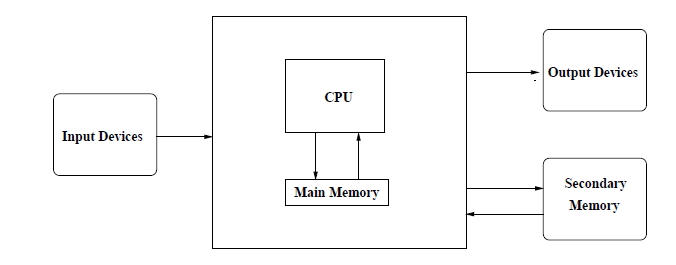
\includegraphics[scale=0.63]{cpu.png}
\end{figure}
\end{center}

\end{frame}

\begin{frame}{Cosas Básicas sobre el Hardware}

\begin{itemize}
\item
  La memoria almacena programas y datos. La CPU puede solo acceder
  directamente a información que está almacenada en la memoria principal
  (Memoria RAM (Random Access Memory)), esta memoria es rápida pero es
  también volátil, es decir, si el computador se llega a apagar la
  información en la memoria se pierde
\item
  Con esto debe existir una memoria secundaria que dé almacenamiento
  permanente, en un computador moderno, es usual encontrar algún tipo de
  medios magnéticos como disco duro (hard drive), medios óptico como CD
  (Compact disc) y DVD (Digital Versatile Disc) y memorias flash como
  memoria ``USB'' (stick memory)
\end{itemize}

\end{frame}

\begin{frame}{Cosas Básicas sobre el Hardware}

\begin{itemize}
\item
  los humanos interactuan con el computador a través de dispositivos de
  entrada y salida, dispositivos como el mouse, teclado son dispositivos
  de entrada.
\item
  Tecnicamente la CPU sigue un proceso llamado ciclo Búsqueda-ejecución
  (fetch-execute cycle). La primera instrucción es recuperada de la
  memoria, descifrada para descubrir lo que representa y la acción
  apropiada es llevada a cabo. Entonces la siguiente instrucción es
  traída, decodificada y ejecutada. El ciclo continua instrucción tras
  instrucción. Esto es realmente lo que hace un computador desde que se
  enciende hasta que se apaga, para algo trivial pero la velocidad y la
  cantidad de millones de instrucciones que mueve la memoria cada
  segundo es impresionanante
\end{itemize}

\end{frame}

\begin{frame}{Lenguajes de Programación}

\begin{itemize}
\item
  Recordando que un programa es solo una secuencia de instrucciones que
  le dicen a un computador que hacer. Obviamente, necesitamos proveer
  esas instrucciones en un lenguaje que el computador puede entender.
  Sería genial si se pudiera indicarle a un computador usando el
  lenguaje nativo pero a pesar de los esfuerzo, diseñar un computador
  que pueda entender el lenguaje humano es una tarea sin solución, pues
  el lenguaje natural es tenso con ambiguedades e imprecisiones
\item
  Las científicos en computación han conseguido alrededor de este
  problema diseñar notaciones para experesar cálculos en una vía exacta
  y sin ambiguedades. Estas notaciones especiales son llamadas lenguajes
  de programación
\end{itemize}

\end{frame}

\begin{frame}{Lenguajes de Programación}

\begin{itemize}
\item
  Toda estructura en un leguaje de programación tiene una forma precisa
  (sintaxis) y un significado preciso (semántica)
\item
  Los programadores se refieren a menudo a sus programam como un código
  de computadora
\item
  y el proceso de escribir un algoritmo en un leguaje de progrmación se
  denomina codificar
\end{itemize}

\end{frame}

\begin{frame}{Lenguajes de Programación}

\begin{itemize}
\item
  R es un ejemplo de un lenguaje de programación y el que veremos
  durante todo el curso
\item
  Existen otro tipo de lenguaje como Python, Java, C++, Fortran, Basic.
  Los cuales poseen diferente características pero comparten la
  característica de estar bien definidos, sintaxis y semántica no
  ambiguas
\item
  los lenguajes mencionados anteriormente son ejemplos de lenguajes de
  alto nivel, los cuales, además de ser precisos, son diseñados para ser
  usados y entendido por humanos
\end{itemize}

\end{frame}

\begin{frame}{Lenguajes de Programación}

\begin{itemize}
\item
  El hardware computacional puede solo entender un muy lenguaje de bajo
  de nivel conocido como lenguaje de máquina
\item
  Suponga que queremos que el computador sume dos números. La
  instrucción que la CPU lleva a cabo realmente puede ser algo como
\end{itemize}

\end{frame}

\begin{frame}{Lenguajes de Programación}

\begin{itemize}
\item
  cargue el número desde la ubicación 2001 en memoria a la CPU
\item
  cargue el número desde la ubicación 2002 en memoria a la CPU
\item
  sume los dos números en la CPU
\item
  Almacene los dos números en la ubicación 2003
\end{itemize}

Parece ser mucho trbajo sumar dos número, es más, puede ser más
complicado sabiendo que la instrucción y los números son representados
en notación binaria

\end{frame}

\begin{frame}{Lenguajes de Programación}

\begin{itemize}
\item
  En un lenguaje de alto nivel la suma de dos números se puede hacer de
  una simple manera c = a + b que es más fácil de entender, pero
  necesitamos transladar esto a un lenguaje de máquina que el computador
  pueda ejecutar, para esto disponemos de dos maneras compilar o
  interpretar
\item
  Un compilador es un programa de computadora complejo que toma otro
  programa escrito en alto nivel y lo traduce a un equivalente programa
  en lenguaje de máquina de algún computador
\end{itemize}

\end{frame}

\begin{frame}{Lenguajes de Programación}

\begin{center}
\begin{figure}
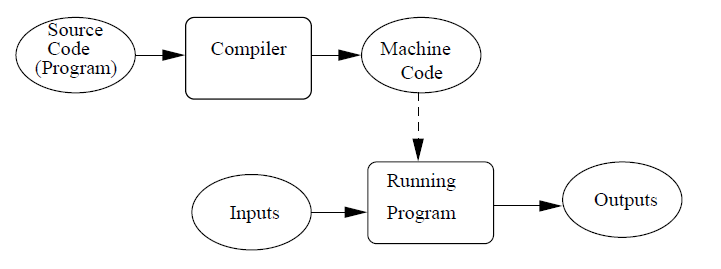
\includegraphics[scale=0.63]{compilado.png}
\end{figure}
\end{center}

\end{frame}


\begin{frame}{Lenguajes de Programación}

\begin{itemize}
\item
  Un interpetador es un programa que simula una computadora que entiende
  un leguaje de alto nivel. En vez de traducir, el programa fuente a
  lenguaje de máquina equivalente, el interpretador analiza y ejecuta la
  instrucción de código fuente instrucción por instrucción cuante veces
  sea necesario
\item
  La diferencia entre interpretador y compilador es que un compilador es
  una traducción de un tiro, una vez el programa es compilado, este
  puede ser corrido una y otra vez sin más trabajo del compilador o el
  código fuente. En el caso de un interpretador, la interpretación y el
  código fuente son necesarias cada vez que se corre el programa
\end{itemize}

\end{frame}

\begin{frame}{Lenguajes de Programación}

\begin{center}
\begin{figure}
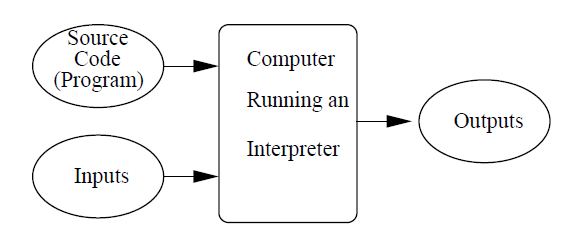
\includegraphics[scale=0.63]{interpretado.png}
\end{figure}
\end{center}

\end{frame}

\begin{frame}{Lenguajes de Programación}

\begin{itemize}
\item
  los programas compilados tienden a ser más rápidos, pero los lenguajes
  interpretados tienden a si mismos a tener un ambiente de programamción
  más flexible, como programa que pueden ser desarrollados y corridos
  interactivamente
\item
  otra ventaja en los programas de alto nivel es su portabilidad y es
  que estos puede correr en cualquier CPU, contrario a los lenguajes de
  máquina los cuales pueden ser corrido para CPU de sus respectivos
  fabricantes
\end{itemize}

\end{frame}

\begin{frame}{R}

\begin{center}
\begin{figure}

\includegraphics[scale=0.9]{r.png}
\end{figure}
\end{center}

\end{frame}


\begin{frame}{Introducción a R (Definición)}

\begin{itemize}
\tightlist
\item
  De esta manera, R es un leguaje de alto nivel y un ambiente de trabajo
  para el análisis de datos y gráficos, este posee un intérprete el cual
  ejecuta el código que le demos, a diferencia de lenguajes como Java, C
  o C++ los cuales deben compilar primero su código, aunque en algunos
  Códigos exigentes son escritos en C o C++.
\end{itemize}

\end{frame}

\begin{frame}{Introducción a R (Origen)}

\begin{itemize}
\item
  R es un software de libre uso y distribución bajo Licencia Pública
  General de GNU, para programar análisis estadístico y gráfico. R fue
  creado en 1993 por Robert Gentleman y Ross Ihaka del Departamento de
  Estadística de la Universidad de Auckland-Nueva Zelanda y desde 1997
  se desarrolla con aportes de diversas partes del mundo, bajo la
  coordinación del equipo principal de desarrollo de R (R Core Team
  Development) (R Project).
\item
  Es un programa clonado del program S-Plus
\end{itemize}

\end{frame}

\begin{frame}{¿Por qué usar R?}

\begin{itemize}
\item
  Primero que todo R es Gratis y es de código abierto, es decir, es un
  proyecto colaborativo y abierto donde los usuarios pueden definir sus
  propias funciones, aparte de numerosas biblioteca preconstruidas que
  tiene, también se pueden publicar paquetes que puede extender su
  configuración básica
\item
  Es posible que algoritmos computacionalmente exigentes pueden ser
  desarrollados en C, C++ o Fortran y vincularlos directamente con R
\item
  Al ser un lenguaje que contiene interpretador posee variedad de
  ambientes de trabajo como R Studio, R Commander, Tinn R y el ambiente
  predeterminado que permiten una amigabilidad a la hora de manejar
  códigos y datos
\end{itemize}

\end{frame}

\begin{frame}{¿Por qué usar R?}

\begin{itemize}
\tightlist
\item
  R funciona con paquetes de programación, los cuales están disponibles
  en una Red Comprehensiva de Archivos R (Comprehensive R Archive
  Network, CRAN) en sitios web llamados MIRROR- sitios que contienen
  réplicas exactas de R- desde los cuales los usuarios finales pueden
  descargarlos. Actualmente están disponibles 92 CRAN-MIRROR, en 45
  países de los cinco continentes, 14 de las cuales se encuentran en
  instituciones - principalmente universidades- de siete países de
  América Latina: Argentina, Brasil, Chile, Colombia, Ecuador, México y
  Venezuela
\end{itemize}

\end{frame}

\begin{frame}{Propiedades de R (Funcional)}

\begin{itemize}
\item
  Las funciones en R se pueden manipular igual que los vectores. Además
  puedes asignar las funciones a variables, almacenarlas en listas,
  devolverlas como resultados de otras funciones o incluso pasarlas como
  argumentos de otras funciones
\item
  Ofrece múltiples posibilidades para atacar a datos almacenados en
  distintos tipos de bases de datos. También presenta múltiples bindings
  y paquetes que permiten a R interactuar con otros lenguajes (como
  Perl, Ruby o Python) e intercambiar objetos con ellos.
\item
  Existen librerías para R que permiten generar una extensa variedad de
  gráficos, desde la completísima ggplot2 hasta otras más simples pero
  también potentes como corrplot
\end{itemize}

\end{frame}

\begin{frame}{¿Por qué usar R?}

\begin{itemize}
\item
  R mantiene todos los objetos que definimos en nuestro programa en la
  memoria de nuestra máquina. Por ello, es importante entender cómo
  gestiona la memoria, para poder optimizar nuestro código. Así
  evitamos, por ejemplo, copias innecesarias de objetos que pueden
  ralentizarlo y hacer llegar a un límite nuestra máquina.
\item
  Este lenguaje de programación fue concebido para el análisis
  estadístico, aunque también se utiliza en la minería y análisis de
  datos, investigación biomédica, bioinformática, machine
  learning\ldots{} Esto es porque proporciona un amplio abanico de
  herramientas estadísticas y gráficas, además de tener una gran
  potencia como herramienta de cálculo.
\end{itemize}

\end{frame}

\begin{frame}{Instalación}

\begin{itemize}
\item
  \url{http://cran.r-project.org/}
\item
  R Studio
\end{itemize}

\end{frame}

\begin{frame}[fragile]{Iniciar R}

\begin{Shaded}
\begin{Highlighting}[]
\CommentTok{#R version 3.5.1 (2018-07-02) -- "Feather Spray"}
\CommentTok{#Copyright (C) 2018 The R Foundation for Statistical   Computing}
\CommentTok{#Platform: x86_64-w64-mingw32/x64 (64-bit)}

\CommentTok{#R is free software and comes with ABSOLUTELY NO WARRANTY.}
\CommentTok{#You are welcome to redistribute it under certain #conditions.}
\CommentTok{#Type 'license()' or 'licence()' for distribution details.}

\CommentTok{#R is a collaborative project with many contributors.}
\CommentTok{#Type 'contributors()' for more information and}
\CommentTok{#'citation()' on how to cite R or R packages in publications.}

\CommentTok{#Type 'demo()' for some demos, 'help()' for on-line help, or}
\CommentTok{#'help.start()' for an HTML browser interface to help.}
\CommentTok{#Type 'q()' to quit R.}
\end{Highlighting}
\end{Shaded}

\end{frame}

\begin{frame}{Iniciar R}

Debajo de este encabezado veremos una línea impresa con \textgreater{}
de símbolo en la parte izquierda del margen. Este es llamado el prompt y
es el lugaro donde escribiremos nuestros comando. Cuando trabajama
algunas veces veremos un símbolo como + el la parte izpuierda del
margen, lo que indicará que el comando escrito no está completo.

Podremos ejecutar los comando oprimiendo Enter y si cometes un error
oprimiendo Esc se logrará retornar al prompt

\end{frame}

\begin{frame}{The Comprehensive R Archive Network (CRAN)}

Es nuestro primer sitio par acudir y llamar cualquier cosa que queramos
hacer en R, es desde aquí que podemos descargar, instalar R, encontrar
ppaquetes para resolver cierto problemas y encontrar las respuestas y
hacer preguntas acerca de los últimos desarrollos

\begin{itemize}
\tightlist
\item
  \url{http://cran.r-project.org/}
\end{itemize}

\end{frame}

\begin{frame}[fragile]{Obtener ayuda en R}

Si tienes el nombre específico de la función

\begin{Shaded}
\begin{Highlighting}[]
\CommentTok{?read.table}
\end{Highlighting}
\end{Shaded}

Si no tienes el nombre de la función pero sabes el tema con el que
tratas

\begin{Shaded}
\begin{Highlighting}[]
\KeywordTok{help.search}\NormalTok{(}\StringTok{"data input"}\NormalTok{)}
\end{Highlighting}
\end{Shaded}

\end{frame}

\begin{frame}[fragile]{Obtener ayuda en R}

para encontrar el paquete correspondiente a una función

\begin{Shaded}
\begin{Highlighting}[]
\KeywordTok{find}\NormalTok{(}\StringTok{"lowess"}\NormalTok{)}
\end{Highlighting}
\end{Shaded}

\begin{verbatim}
## [1] "package:stats"
\end{verbatim}

para encorntrar ciertos elementos asociados a una función o palabra que
estemos buscando

\begin{Shaded}
\begin{Highlighting}[]
\KeywordTok{apropos}\NormalTok{(}\StringTok{"lm"}\NormalTok{)}
\end{Highlighting}
\end{Shaded}

\end{frame}

\begin{frame}[fragile]{Obtener ayuda en R}

Para ver ejemplos asociados a las funciones

\begin{Shaded}
\begin{Highlighting}[]
\KeywordTok{example}\NormalTok{(}\StringTok{lm}\NormalTok{)}
\end{Highlighting}
\end{Shaded}

demostraciones

\begin{Shaded}
\begin{Highlighting}[]
\KeywordTok{demo}\NormalTok{(}\StringTok{persp}\NormalTok{)}
\KeywordTok{demo}\NormalTok{(}\StringTok{graphics}\NormalTok{)}
\KeywordTok{demo}\NormalTok{(}\StringTok{Hershey}\NormalTok{)}
\KeywordTok{demo}\NormalTok{(}\StringTok{plotmath}\NormalTok{)}
\end{Highlighting}
\end{Shaded}

\end{frame}

\begin{frame}[fragile]{Paquetes}

Encontrar paquetes que han sido contibuídos en R puede ser una tarea
ardua, además que no siempre el nombre del paquete es una vía para
encontrar cierta función; para esto R tiene asignados los paquetes por
ciertas categorías que pueden ser visualizadas en el CRAN

\begin{itemize}
\tightlist
\item
  \url{http://cran.r-project.org/} -\textgreater{} Task Views
\end{itemize}

Para poder usar uno de los paquetes previamente descargardos usamos la
función library

\begin{Shaded}
\begin{Highlighting}[]
\KeywordTok{library}\NormalTok{(spatial)}
\end{Highlighting}
\end{Shaded}

\end{frame}

\begin{frame}[fragile]{Paquetes}

Usando la ayuda de R podemos descubrir los contenidos de libraría de los
paquetes así

\begin{Shaded}
\begin{Highlighting}[]
\KeywordTok{library}\NormalTok{(}\StringTok{help=spatial}\NormalTok{)}
\end{Highlighting}
\end{Shaded}

Puedes ver una lista de los contenidos de una librería usando objects
con search()

\end{frame}

\begin{frame}[fragile]{Paquetes}

\begin{Shaded}
\begin{Highlighting}[]
\KeywordTok{objects}\NormalTok{(}\KeywordTok{grep}\NormalTok{(}\StringTok{"spatial"}\NormalTok{,}\KeywordTok{search}\NormalTok{()))}
\end{Highlighting}
\end{Shaded}

\begin{verbatim}
##  [1] "anova.trls"     "anovalist.trls" "correlogram"    "expcov"        
##  [5] "gaucov"         "Kaver"          "Kenvl"          "Kfn"           
##  [9] "plot.trls"      "ppgetregion"    "ppinit"         "pplik"         
## [13] "ppregion"       "predict.trls"   "prmat"          "Psim"          
## [17] "semat"          "sphercov"       "SSI"            "Strauss"       
## [21] "surf.gls"       "surf.ls"        "trls.influence" "trmat"         
## [25] "variogram"
\end{verbatim}

\end{frame}

\begin{frame}[fragile]{Paquetes}

Para instalar paquetes usamos

\begin{Shaded}
\begin{Highlighting}[]
\KeywordTok{install.packages}\NormalTok{(}\StringTok{"tree"}\NormalTok{)}
\end{Highlighting}
\end{Shaded}

\end{frame}

\begin{frame}{Línea de Comando versus scrpits}

Cuando escribimos funciones y otras secciones multi-línea de salida,
algunas personas le encuentran más utilidad en usar un editor de texto
en vez de ejecutar directamente todo directamente en la línea de
comando. Muchas personas prefieren usar el ambiente original de R, R
Studio, Tinn-R, etc.

Para correr ciertas líneas desde un script, se seleccionana y se oprime
Ctrl+R y las líneas son automáticamente tranferidas a la línea de
comando.

Para guardar usamos Ctrl+S se guerdan la ventana editor en un archivo
con extensión .R

\end{frame}

\begin{frame}[fragile]{Buena limpieza}

Para ver que variables ha creado en su actual sesión usamos

\begin{Shaded}
\begin{Highlighting}[]
\KeywordTok{objects}\NormalTok{()}
\end{Highlighting}
\end{Shaded}

para ver que paquetes y dataframes se ha usado

\begin{Shaded}
\begin{Highlighting}[]
\KeywordTok{search}\NormalTok{()}
\end{Highlighting}
\end{Shaded}

\begin{verbatim}
##  [1] ".GlobalEnv" "package:spatial" "package:stats"    
##  [4] "package:graphics" "package:grDevices" "package:utils"    
##  [7] "package:datasets" "package:methods" "Autoloads"        
## [10] "package:base"
\end{verbatim}

\end{frame}

\begin{frame}[fragile]{Buena limpieza}

para eliminar variables usamos

\begin{Shaded}
\begin{Highlighting}[]
\KeywordTok{rm}\NormalTok{()}
\end{Highlighting}
\end{Shaded}

El comando detach no desaparece una variable, solo hace que las
variables del dataframe no estén accesibles de manera directa

\begin{Shaded}
\begin{Highlighting}[]
\KeywordTok{detach}\NormalTok{()}
\end{Highlighting}
\end{Shaded}

\end{frame}

\begin{frame}[fragile]{Buena limpieza}

para deshacerse de todo incluyendo dataframes usamos

\begin{Shaded}
\begin{Highlighting}[]
\KeywordTok{rm}\NormalTok{(}\StringTok{list=ls()}\NormalTok{)}
\end{Highlighting}
\end{Shaded}

\end{frame}

\begin{frame}{Apartes del Curso}

\begin{itemize}
\tightlist
\item
  1er Corte:

  \begin{itemize}
  \tightlist
  \item
    parcial (14 marzo): 40\%
  \item
    Taller: 15\%
  \item
    Quiz: 25\%
\item
    Lectura (21 marzo): 10\%
\item
    Pre-anteproyecto (14 marzo): 10\%
  \end{itemize}
\item
  2do Corte:

  \begin{itemize}
  \tightlist
  \item
    parcial (25 abril): 40\%
  \item
    Taller: 20\%
  \item
    Quiz: 30\%
  \item
     Propuesta proyecto final (25 abril): 10 \%
  \end{itemize}
\item
  3er Corte:

  \begin{itemize}
  \tightlist
  \item
    Quiz: 40\%
  \item
    Proyecto Final (29 y 30 mayo): 60\%
  \end{itemize}
\end{itemize}

\end{frame}

\end{document}
